

\tikzset{every picture/.style={line width=0.75pt}} %

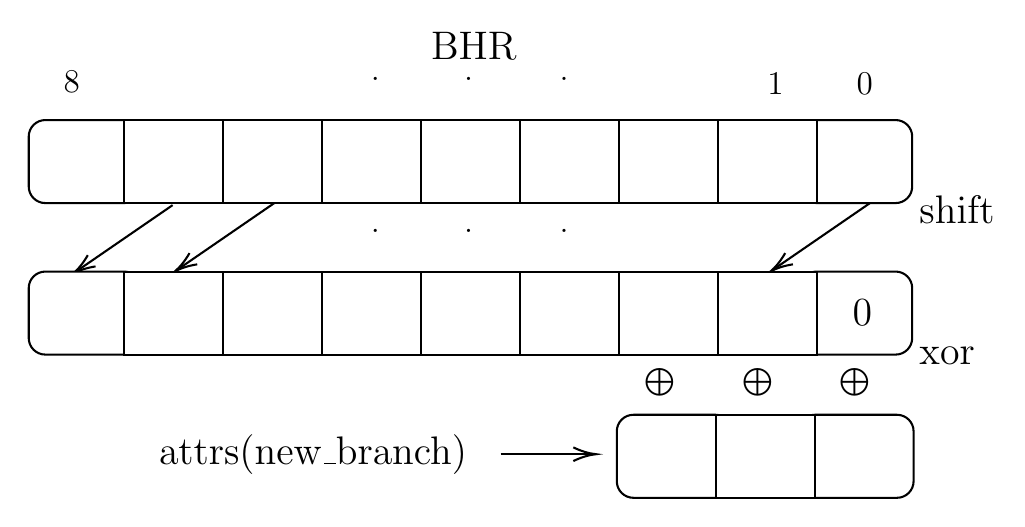
\begin{tikzpicture}[x=0.75pt,y=0.75pt,yscale=-1,xscale=1]

\draw  [fill={rgb, 255:red, 255; green, 255; blue, 255 }  ,fill opacity=1 ] (208.33,400) -- (256,400) -- (256,440) -- (208.33,440) -- cycle ;
\draw  [fill={rgb, 255:red, 255; green, 255; blue, 255 }  ,fill opacity=1 ] (256,400) -- (303.67,400) -- (303.67,440) -- (256,440) -- cycle ;
\draw  [fill={rgb, 255:red, 255; green, 255; blue, 255 }  ,fill opacity=1 ] (303.67,400) -- (351.33,400) -- (351.33,440) -- (303.67,440) -- cycle ;
\draw  [fill={rgb, 255:red, 255; green, 255; blue, 255 }  ,fill opacity=1 ] (351.33,400) -- (399,400) -- (399,440) -- (351.33,440) -- cycle ;
\draw  [fill={rgb, 255:red, 255; green, 255; blue, 255 }  ,fill opacity=1 ] (399,400) -- (446.67,400) -- (446.67,440) -- (399,440) -- cycle ;
\draw  [fill={rgb, 255:red, 255; green, 255; blue, 255 }  ,fill opacity=1 ] (114.67,408) .. controls (114.67,403.58) and (118.25,400) .. (122.67,400) -- (160.67,400) .. controls (165.08,400) and (168.67,403.58) .. (168.67,408) -- (168.67,432) .. controls (168.67,436.42) and (165.08,440) .. (160.67,440) -- (122.67,440) .. controls (118.25,440) and (114.67,436.42) .. (114.67,432) -- cycle ;
\draw  [fill={rgb, 255:red, 255; green, 255; blue, 255 }  ,fill opacity=1 ] (160.67,400) -- (208.33,400) -- (208.33,440) -- (160.67,440) -- cycle ;
\draw  [fill={rgb, 255:red, 255; green, 255; blue, 255 }  ,fill opacity=1 ] (486.33,408) .. controls (486.33,403.58) and (489.92,400) .. (494.33,400) -- (532.33,400) .. controls (536.75,400) and (540.33,403.58) .. (540.33,408) -- (540.33,432) .. controls (540.33,436.42) and (536.75,440) .. (532.33,440) -- (494.33,440) .. controls (489.92,440) and (486.33,436.42) .. (486.33,432) -- cycle ;
\draw  [fill={rgb, 255:red, 255; green, 255; blue, 255 }  ,fill opacity=1 ] (446.67,400) -- (494.33,400) -- (494.33,440) -- (446.67,440) -- cycle ;

\draw    (184,441) -- (137.65,472.87) ;
\draw [shift={(136,474)}, rotate = 325.49] [color={rgb, 255:red, 0; green, 0; blue, 0 }  ][line width=0.75]    (10.93,-3.29) .. controls (6.95,-1.4) and (3.31,-0.3) .. (0,0) .. controls (3.31,0.3) and (6.95,1.4) .. (10.93,3.29)   ;
\draw    (233,440) -- (186.65,471.87) ;
\draw [shift={(185,473)}, rotate = 325.49] [color={rgb, 255:red, 0; green, 0; blue, 0 }  ][line width=0.75]    (10.93,-3.29) .. controls (6.95,-1.4) and (3.31,-0.3) .. (0,0) .. controls (3.31,0.3) and (6.95,1.4) .. (10.93,3.29)   ;
\draw    (520,440) -- (473.65,471.87) ;
\draw [shift={(472,473)}, rotate = 325.49] [color={rgb, 255:red, 0; green, 0; blue, 0 }  ][line width=0.75]    (10.93,-3.29) .. controls (6.95,-1.4) and (3.31,-0.3) .. (0,0) .. controls (3.31,0.3) and (6.95,1.4) .. (10.93,3.29)   ;
\draw  [fill={rgb, 255:red, 255; green, 255; blue, 255 }  ,fill opacity=1 ] (208.33,473) -- (256,473) -- (256,513) -- (208.33,513) -- cycle ;
\draw  [fill={rgb, 255:red, 255; green, 255; blue, 255 }  ,fill opacity=1 ] (256,473) -- (303.67,473) -- (303.67,513) -- (256,513) -- cycle ;
\draw  [fill={rgb, 255:red, 255; green, 255; blue, 255 }  ,fill opacity=1 ] (303.67,473) -- (351.33,473) -- (351.33,513) -- (303.67,513) -- cycle ;
\draw  [fill={rgb, 255:red, 255; green, 255; blue, 255 }  ,fill opacity=1 ] (351.33,473) -- (399,473) -- (399,513) -- (351.33,513) -- cycle ;
\draw  [fill={rgb, 255:red, 255; green, 255; blue, 255 }  ,fill opacity=1 ] (399,473) -- (446.67,473) -- (446.67,513) -- (399,513) -- cycle ;
\draw  [fill={rgb, 255:red, 255; green, 255; blue, 255 }  ,fill opacity=1 ] (114.67,481) .. controls (114.67,476.58) and (118.25,473) .. (122.67,473) -- (160.67,473) .. controls (165.08,473) and (168.67,476.58) .. (168.67,481) -- (168.67,505) .. controls (168.67,509.42) and (165.08,513) .. (160.67,513) -- (122.67,513) .. controls (118.25,513) and (114.67,509.42) .. (114.67,505) -- cycle ;
\draw  [fill={rgb, 255:red, 255; green, 255; blue, 255 }  ,fill opacity=1 ] (160.67,473) -- (208.33,473) -- (208.33,513) -- (160.67,513) -- cycle ;
\draw  [fill={rgb, 255:red, 255; green, 255; blue, 255 }  ,fill opacity=1 ] (486.33,481) .. controls (486.33,476.58) and (489.92,473) .. (494.33,473) -- (532.33,473) .. controls (536.75,473) and (540.33,476.58) .. (540.33,481) -- (540.33,505) .. controls (540.33,509.42) and (536.75,513) .. (532.33,513) -- (494.33,513) .. controls (489.92,513) and (486.33,509.42) .. (486.33,505) -- cycle ;
\draw  [fill={rgb, 255:red, 255; green, 255; blue, 255 }  ,fill opacity=1 ] (446.67,473) -- (494.33,473) -- (494.33,513) -- (446.67,513) -- cycle ;
\draw  [fill={rgb, 255:red, 255; green, 255; blue, 255 }  ,fill opacity=1 ] (398,550) .. controls (398,545.58) and (401.58,542) .. (406,542) -- (445.67,542) .. controls (450.08,542) and (453.67,545.58) .. (453.67,550) -- (453.67,574) .. controls (453.67,578.42) and (450.08,582) .. (445.67,582) -- (406,582) .. controls (401.58,582) and (398,578.42) .. (398,574) -- cycle ;
\draw  [fill={rgb, 255:red, 255; green, 255; blue, 255 }  ,fill opacity=1 ] (485.33,550) .. controls (485.33,545.58) and (488.92,542) .. (493.33,542) -- (533,542) .. controls (537.42,542) and (541,545.58) .. (541,550) -- (541,574) .. controls (541,578.42) and (537.42,582) .. (533,582) -- (493.33,582) .. controls (488.92,582) and (485.33,578.42) .. (485.33,574) -- cycle ;
\draw  [fill={rgb, 255:red, 255; green, 255; blue, 255 }  ,fill opacity=1 ] (445.67,542) -- (493.33,542) -- (493.33,582) -- (445.67,582) -- cycle ;


\draw    (342,561) -- (386,561) ;
\draw [shift={(388,561)}, rotate = 180] [color={rgb, 255:red, 0; green, 0; blue, 0 }  ][line width=0.75]    (10.93,-3.29) .. controls (6.95,-1.4) and (3.31,-0.3) .. (0,0) .. controls (3.31,0.3) and (6.95,1.4) .. (10.93,3.29)   ;


\draw (369,451) node [anchor=north west][inner sep=0.75pt]   [align=left] {\textbf{{\large {\fontfamily{helvet}\selectfont .}}}};
\draw (323,451) node [anchor=north west][inner sep=0.75pt]   [align=left] {\textbf{{\large {\fontfamily{helvet}\selectfont .}}}};
\draw (278,451) node [anchor=north west][inner sep=0.75pt]   [align=left] {\textbf{{\large {\fontfamily{helvet}\selectfont .}}}};
\draw (369,378) node [anchor=north west][inner sep=0.75pt]   [align=left] {\textbf{{\large {\fontfamily{helvet}\selectfont .}}}};
\draw (323,378) node [anchor=north west][inner sep=0.75pt]   [align=left] {\textbf{{\large {\fontfamily{helvet}\selectfont .}}}};
\draw (278,378) node [anchor=north west][inner sep=0.75pt]   [align=left] {\textbf{{\large {\fontfamily{helvet}\selectfont .}}}};
\draw (469,376) node [anchor=north west][inner sep=0.75pt]   [align=left] {{\large \textbf{{\fontfamily{helvet}\selectfont 1}}}};
\draw (512,376) node [anchor=north west][inner sep=0.75pt]   [align=left] {{\large \textbf{{\fontfamily{helvet}\selectfont 0}}}};
\draw (130,375) node [anchor=north west][inner sep=0.75pt]   [align=left] {{\large \textbf{{\fontfamily{helvet}\selectfont 8}}}};
\draw (307,356) node [anchor=north west][inner sep=0.75pt]   [align=left] {\textbf{{\fontfamily{helvet}\selectfont {\Large BHR}}}};
\draw (251.63,561.11) node   [align=left] {\begin{minipage}[lt]{130.05pt}\setlength\topsep{0pt}
\begin{center}

\textbf{{\fontfamily{helvet}\selectfont {\Large attrs(new\_branch)}}}

\end{center}

\end{minipage}};
\draw (410,518.4) node [anchor=north west][inner sep=0.75pt]    {$\bigoplus $};
\draw (457,518.4) node [anchor=north west][inner sep=0.75pt]    {$\bigoplus $};
\draw (542.33,435) node [anchor=north west][inner sep=0.75pt]   [align=left] {\textbf{{\fontfamily{helvet}\selectfont {\Large shift}}}};
\draw (542.33,508) node [anchor=north west][inner sep=0.75pt]   [align=left] {\textbf{{\fontfamily{helvet}\selectfont {\Large xor}}}};
\draw (504,518.4) node [anchor=north west][inner sep=0.75pt]    {$\bigoplus $};
\draw (516.34,493) node   [align=left] {{\Large \textbf{{\fontfamily{helvet}\selectfont 0}}}};


\end{tikzpicture}
